%%%%%%%%%%%%%%%%%%%%%%%%%%%%%%%%%%%%%%%%%
% Memo
% LaTeX Template
% Version 1.0 (30/12/13)
%
% This template has been downloaded from:
% http://www.LaTeXTemplates.com
%
% Original author:
% Rob Oakes (http://www.oak-tree.us) with modifications by:
% Vel (vel@latextemplates.com)
%
% License:
% CC BY-NC-SA 3.0 (http://creativecommons.org/licenses/by-nc-sa/3.0/)
%
%%%%%%%%%%%%%%%%%%%%%%%%%%%%%%%%%%%%%%%%%

\documentclass[letterpaper,11pt]{texMemo} % Set the paper size (letterpaper, a4paper, etc) and font size (10pt, 11pt or 12pt)

\usepackage{fancyhdr}
\usepackage{fancybox}
\usepackage{longtable}
\usepackage{amsmath}
%----------------------------------------------------------------------------------------
%	MEMO INFORMATION
%----------------------------------------------------------------------------------------

\memoto{Luis Andr\'es Valido Fajardo. luis.valido@umcc.cu (53694742)} % Recipient(s)

\memofrom{Josval Díaz Blanco} % Sender(s)

\memosubject{Guía de Aprendizaje para Concursantes ICPC y IOI: Búsqueda Binaria } % Memo subject

\memodate{\today} % Date, set to \today for automatically printing todays date

\logo{
\includegraphics[scale=0.5]{img/icpc}} % Institution logo at the top right of the memo, comment out this line for no logo

%----------------------------------------------------------------------------------------

\begin{document}

%\AddToShipoutPicture{\BackgroundPic}
\maketitle % Print the memo header information
%\tableofcontents
\pagestyle{plain}
\pagebreak

\pagestyle{fancy}
\fancyhead[LO,CE]{ }
\fancyhead[RO,CE]{
\includegraphics[scale=0.1]{img/icpc}}
\fancyfoot[LO,CE]{\textbf{Autor:} Luis Andrés Valido Fajardo \\ \textbf{Email:} luis.valido1989@gmail.com \\ \textbf{Teléfono:} 53694742}
\fancyfoot[RO,CE]{\emph{Existen 10 tipos de personas Las que \\saben binario y LAS QUE NO}}
\fancypagestyle{plain}{\pagestyle{fancy}}



%\lhead{ }
%\rhead{  }

%\fancyfoot[L]{}
%\fancyfoot[R]{\textbf{Autor:} Luis Andrés Valido Fajardo \\ \textbf{Email:} luis.valido@umcc.cu}
%----------------------------------------------------------------------------------------
%	MEMO CONTENT
%----------------------------------------------------------------------------------------


\section{Introducción}
El diámetro de árbol se define como la longitud máxima que existe entre cualquier par de nodos que integren el árbol. Para poder calcular esta propiedad el árbol que se vaya analizar tiene que ser no dirigido y la aristas con un peso no negativo. Por ejemplo, considere el siguiente árbol:

% TODO: \usepackage{graphicx} required
\begin{figure}[h!]
	\centering
	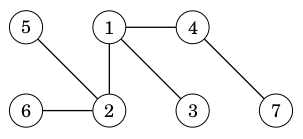
\includegraphics[width=0.5\linewidth]{img/diameter_tree_1}
	\label{fig:diametertree1}
\end{figure}

El diámetro de este árbol es 4, lo que corresponde al siguiente camino:

\begin{figure}[h!]
	\centering
	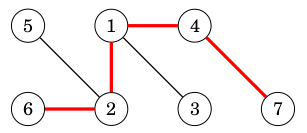
\includegraphics[width=0.5\linewidth]{img/diameter_tree_2}
	\label{fig:diametertree2}
\end{figure}

Tenga en cuenta que puede haber varias rutas de longitud máxima. En la ruta anterior, podríamos reemplazar el nodo 6 con el nodo 5 para obtener otra ruta con longitud 4. La siguiente guía va abordar como determinar el diámetro de un árbol.
\section{Conocimientos previos}
\subsection{Recorrido en Profundidad (\emph{DFS})}
Búsqueda en profundidad. Una Búsqueda en profundidad (en inglés \emph{DFS} o \emph{Depth First Search}) es un algoritmo que permite recorrer todos los nodos de un grafo o árbol (teoría de grafos) de manera ordenada, pero no uniforme. Su funcionamiento consiste en ir expandiendo todos y cada uno de los nodos que va localizando, de forma recurrente, en un camino concreto. Cuando ya no quedan más nodos que visitar en dicho camino, regresa (Backtracking), de modo que repite el mismo proceso con cada uno de los hermanos del nodo ya procesado. 

\subsection{Programación Dinámica}
La programación dinámica es un método para reducir el tiempo de ejecución de un algoritmo mediante la utilización de subproblemas superpuestos y subestructuras óptimas. 
\section{Desarrollo}
Una idea muy trivial para solucionar el problema pudiera ser para cada nodo del árbol buscar buscar su nodo mas alejado y la solución sería aquel par de nodos cuya distancia entre ellos fuera mayor. Esto lo pudieramos realizar aplicando un dfs por cada nodo lo cual podría tener una complejidad de O($VE$) siendo $V$ la cantidad de nodos y $E$ la cantidad de aristas del árbol, pero como la cantidad de aristas de un árbol es igual a $V-1$ la complejidad de esta solución quedaría O($V^2-V$). Pero esta idea tan trivial es la que da inicio a la primera variante de solución.

\subsection{Recorrido en Profundidad (\emph{DFS})}

El algoritmo en sí mismo es bastante simple. Se toma un nodo $a$ de forma aleatoria y se explora el resto del árbol usando un dfs y calculando para cada nodo del árbol su distancia con respecto al nodo $a$ . Una vez terminado este primer dfs buscamos que nodo esta más alejado con respecto al nodo $a$  que tomamos de forma aleatoria la primera vez. Al nodo mas alejado del nodo $a$  lo nombraremos nodo $b$ . Ahora a partir del nodo $b$  realizaremos un dfs para buscar el nodo $c$  que va ser el nodo más alejado del nodo $b$ . Una vez hallado el nodo $c$ , podemos decir con seguridad que el par de nodos $b,c$  son los nodos más alejados en el árbol por tanto su distancia entre ellos va a definir el díametro del árbol.

En el siguiente árbol, $a$, $b$ y $c$ podrían ser:

\begin{figure}[h!]
	\centering
	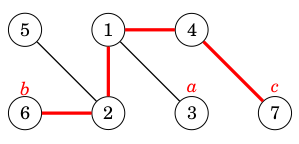
\includegraphics[width=0.5\linewidth]{img/diameter_tree_3}
	\label{fig:diametertree3}
\end{figure}

Este es un método elegante, pero ¿por qué funciona?

Ayuda dibujar el árbol de manera diferente para que el camino que corresponde al diámetro sea horizontal y todos los demás nodos cuelguen de él:

\begin{figure}[h!]
	\centering
	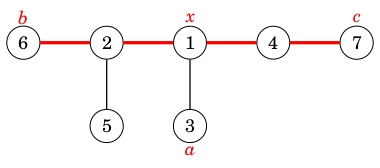
\includegraphics[width=0.5\linewidth]{img/diameter_tree_4}
	\label{fig:diametertree4}
\end{figure}

El nodo $x$ indica el lugar donde el camino del nodo $a$ se une al camino que corresponde al diámetro. El nodo más alejado de $a$ es el nodo $b$, el nodo $c$ o algún otro nodo que esté al menos tan lejos del nodo $x$. Por lo tanto, este nodo es siempre una opción válida para un punto final de una trayectoria que corresponde al diámetro.

\subsection{Programación Dinámica}

Una forma general de abordar muchos problemas de árboles es enraizar primero el árbol de forma arbitraria. Después de esto, podemos intentar resolver el problema por separado para cada subárbol. El siguiente algoritmo para calcular el diámetro se basa en esta idea.

Una observación importante es que cada camino en un árbol enraizado tiene un punto más alto: el nodo más alto que pertenece al camino. Así, podemos calcular para cada nodo la longitud del camino más largo cuyo punto más alto es el nodo. Uno de esos caminos corresponde al diámetro del árbol.

Por ejemplo, en el siguiente árbol, el nodo 1 es el punto más alto del camino que corresponde al diámetro:

\begin{figure}[h!]
	\centering
	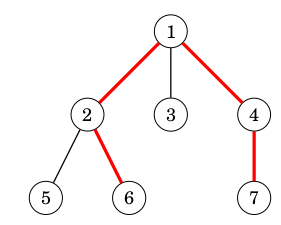
\includegraphics[width=0.5\linewidth]{img/diameter_tree_5}
	\label{fig:diametertree5}
\end{figure}

Calculamos para cada nodo $x$ dos valores:

\begin{itemize}
	\item \textbf{toLeaf(x):} La longitud máxima de una ruta desde $x$ a cualquier hoja
	\item \textbf{maxLength(x):} La longitud máxima de un camino cuyo punto más alto es $x$.
\end{itemize}

\section{Implementación}
\subsection{C++}

\subsubsection{Recorrido en profundidad (\emph{DFS})}
\begin{lstlisting}[language=C++]
struct Node{
   int m_dist,m_dfs;
   vector<int> m_neighbors;
   Node(){ m_neighbors.clear(); m_dfs=m_dist=0;}
};

Node graphs[MAX_N];
int nnodes,a,b;

int diameterTree(int _nodeStart){
   int tDiameter=0,nextNode,currentNode,farthestNode=_nodeStart;
   graphs[_nodeStart].m_dist=0;
   graphs[_nodeStart].m_dfs=1;
	
   stack<int> visit;
   visit.push(_nodeStart);
	
   while(!visit.empty()){
      currentNode=visit.top(); visit.pop();
      if(graphs[currentNode].m_dist>tDiameter){
         tDiameter=graphs[currentNode].m_dist;
         farthestNode=currentNode;
      }
      int tNeighbors=graphs[currentNode].m_neighbors.size();
      for(int i=0;i<tNeighbors;i++){
         nextNode=graphs[currentNode].m_neighbors[i];
         if(graphs[nextNode].m_dfs<1){
            graphs[nextNode].m_dfs=1;
            graphs[nextNode].m_dist=graphs[currentNode].m_dist+1;
            if(graphs[nextNode].m_dist>tDiameter){
               tDiameter=graphs[nextNode].m_dist;
               farthestNode=nextNode;
            }
            visit.push(nextNode);
         }
      }
   }
   
   graphs[farthestNode].m_dist=0;
   graphs[farthestNode].m_dfs=2;
   tDiameter=0;
	
   visit.push(farthestNode);
	
   while(!visit.empty()){
      currentNode=visit.top();
      visit.pop();
      if(graphs[currentNode].m_dist>tDiameter){
         tDiameter=graphs[currentNode].m_dist;
         farthestNode=currentNode;
      }
		
      int tNeighbors=graphs[currentNode].m_neighbors.size();
      for(int i=0;i<tNeighbors;i++){
         nextNode=graphs[currentNode].m_neighbors[i];
         if(graphs[nextNode].m_dfs<2){
            graphs[nextNode].m_dfs=2;
            graphs[nextNode].m_dist=graphs[currentNode].m_dist+1;
            if(graphs[nextNode].m_dist>tDiameter){
               tDiameter=graphs[nextNode].m_dist;
               farthestNode=nextNode;
            }
            visit.push(nextNode);
         }
      }
   }
   return tDiameter;
}
\end{lstlisting} 

\subsubsection{Programación Dinámica}
\begin{lstlisting}[language=C++]
struct Node {
   vector<int> children;
   int maxLength,toLeaft;
   Node(){ children.clear(); maxLength=toLeaft=0;}
};

vector<Node> tree;

void diameterTree(int node ,int par, int * diameter){
   vector<int> childList;
   for(int child : tree[node].children)
      if(child != par){
         diameterTree(child,node,diameter);
         tree[node].maxLength=max(tree[node].maxLength,tree[child].maxLength+1);
         childList.push_back(tree[child].f);
	  }
   *diameter = max(*diameter , tree[node].maxLength);
   sort(childList.begin(),childList.end());
   if(childList.size() >= 2){
      tree[node].toLeaft = 2 + childList[childList.size()-1] + childList[childList.size()-2];
      *diameter = max(*diameter , tree[node].toLeaft);
   }
}
\end{lstlisting}

\subsection{Java}

\subsubsection{Recorrido en profundidad (\emph{DFS})}

\begin{lstlisting}[language=Java]
private class Node{
   int m_dist,m_dfs;
   ArrayList<Integer> m_neighbors;
   public Node(){ m_neighbors =new ArrayList<Integer>(); m_dfs=m_dist=0;}
};

public Node [] graphs;

public int diameterTree(int _nodeStart){
   int tDiameter=0,nextNode,currentNode,farthestNode=_nodeStart;
   graphs[_nodeStart].m_dist=0; graphs[_nodeStart].m_dfs=1;
	
   Stack<Integer> visit =new Stack<Integer>();
   visit.push(_nodeStart);
	
   while(!visit.empty()){
      currentNode=visit.pop();
      if(graphs[currentNode].m_dist>tDiameter){
         tDiameter=graphs[currentNode].m_dist;
         farthestNode=currentNode;
      }
		
      int tNeighbors=graphs[currentNode].m_neighbors.size();
      for(int i=0;i<tNeighbors;i++){
         nextNode=graphs[currentNode].m_neighbors.get(i);
         if(graphs[nextNode].m_dfs<1){
            graphs[nextNode].m_dfs=1;
            graphs[nextNode].m_dist=graphs[currentNode].m_dist+1;
            if(graphs[nextNode].m_dist>tDiameter){
               tDiameter=graphs[nextNode].m_dist;
               farthestNode=nextNode;
            }
			visit.push(nextNode);
         }
       }
   }
	
   graphs[farthestNode].m_dist=0; graphs[farthestNode].m_dfs=2;
   tDiameter=0;
	
   visit.push(farthestNode);
	
   while(!visit.empty()){
      currentNode=visit.pop();
      if(graphs[currentNode].m_dist>tDiameter){
         tDiameter=graphs[currentNode].m_dist;
         farthestNode=currentNode;
      }
		
      int tNeighbors=graphs[currentNode].m_neighbors.size();
      for(int i=0;i<tNeighbors;i++){
         nextNode=graphs[currentNode].m_neighbors.get(i);
         if(graphs[nextNode].m_dfs<2){
            graphs[nextNode].m_dfs=2;
            graphs[nextNode].m_dist=graphs[currentNode].m_dist+1;
            if(graphs[nextNode].m_dist>tDiameter){
               tDiameter=graphs[nextNode].m_dist;
               farthestNode=nextNode;
            }
			visit.push(nextNode);
         }
      }
   }
   return tDiameter;
}
	
\end{lstlisting}

\subsubsection{Programación Dinámica}

\begin{lstlisting}[language=Java]
private class Node{
   ArrayList<Integer> children;
   int maxLentgh,toLeaft;

   public Node(){ children =new ArrayList<Integer>(); maxLentgh=toLeaft=0;}
};

public Node [] graphs;

public int diameter;

public void diameterTree(int node ,int par){
   ArrayList<Integer> childList = new ArrayList<Integer>();
	
   for(int child : graphs[node].children)
      if(child != par){
         diameterTree(child , node);
         graphs[node].maxLentgh = Math.max(graphs[node].maxLentgh,graphs[child].maxLentgh+1);
         childList.add(graphs[child].maxLentgh);
      }
   diameter = Math.max(diameter , graphs[node].maxLentgh);
   Collections.sort(childList);
   if(childList.size() >= 2){
      graphs[node].toLeaft = 2+childList.get(childList.size()-1)+childList.get(childList.size()-2);
      diameter = Math.max(diameter,graphs[node].toLeaft);
   }
}
\end{lstlisting}
\section{Aplicaciones}
Algunas de las aplicaciones comunes del diámetro del árbol  son:

\begin{enumerate}
	\item \textbf{Diseño de red:} En las redes de computadoras, el diámetro de una red representa la distancia máxima entre dos nodos cualesquiera. Ayuda a diseñar algoritmos de enrutamiento eficientes y a determinar el rendimiento general de la red.
	\item \textbf{Redes Sociales:}  El diámetro de una red social se puede utilizar para medir el grado de separación entre individuos. Proporciona información sobre la conectividad y la influencia dentro de una red social.
	\item \textbf{Teoría de grafos:} El diámetro de un árbol es una métrica importante en la teoría de grafos. Ayuda a estudiar las propiedades y características de los árboles, como la conectividad, la centralidad y la resiliencia.
	
	\item \textbf{Análisis de datos:} El diámetro de un árbol se puede utilizar para analizar y visualizar estructuras de datos jerárquicas, como taxonomías, jerarquías organizativas y sistemas de archivos. Ayuda a comprender la estructura y las relaciones dentro de los datos.
	
	\item \textbf{Procesamiento de imágenes:} El diámetro de un árbol se puede utilizar en algoritmos de procesamiento de imágenes para el análisis de formas y el reconocimiento de objetos. Ayuda a determinar el tamaño y la escala de los objetos presentes en una imagen.
	
	\item \textbf{Bioinformática:} El diámetro de un árbol filogenético se utiliza para medir la distancia evolutiva entre especies u organismos. Ayuda a comprender las relaciones genéticas y la historia evolutiva.
	
	\item \textbf{Planificación del transporte:} El diámetro de una red de transporte se puede utilizar para optimizar rutas y determinar la eficiencia de los sistemas de transporte. Ayuda a minimizar el tiempo de viaje y la congestión.
	
	\item \textbf{Redes de sensores:} El diámetro de una red de sensores es importante para la recopilación y el enrutamiento eficientes de datos. Ayuda a determinar la cobertura y conectividad de los sensores en la red.
\end{enumerate}

En general, el diámetro de un árbol tiene diversas aplicaciones en diversos campos, desde la informática hasta la biología, y proporciona información sobre la conectividad, la distancia y la estructura.
 


\section{Complejidad}
El algoritmo que utiliza dos dfs tiene una complejidad de O($2E$) ya que realizamos dos dfs pero la constante $2$ no influye por tanto su complejidad es O($E$)  siendo $E$ la cantidad de aristas del árbol que por definición de un árbol va ser igual a la cantidad de nodos del árbol menos uno.
\section{Ejercicios}
A continuación una lista de ejercicios que se pueden resolver aplicando los algoritmos abordados en esta guía:

\begin{itemize}
	\item \href{https://cses.fi/problemset/task/1131}{CSES - Tree Diameter}
\end{itemize}

\end{document}